\section{The ACQ Problem}
\label{problem}

We now discuss the attributed graph model, the $k$-core, and the AC.  In the CS and CD literature, most existing works assume that the underlying graph is undirected~\cite{KDD2010,vldb2015,attr-topic-sigmod2012,attr-www2013}.
We also suppose that an attributed graph $G(V,E)$ is undirected, with vertex set $V$ and edge set $E$. Each vertex $v \in V$ is associated with a set of keywords, $W(v)$. Let $n$ and $m$ be the corresponding sizes of $V$ and $E$. The degree of a vertex $v$ of $G$ is denoted by $deg_G(v)$. Table~\ref{tab:notation} lists the symbols used in the paper.

\begin{table}[]
  \centering \footnotesize \caption {Symbols and meanings.}
  \label{tab:notation}
  \small
  \begin{tabular}{c|l}
     \hline
          {\bf Symbol} & {\bf Meaning}\\
     \hline\hline
          $G(V,E)$       & A graph with vertex set $V$ and edge set $E$\\ %($n$=$|V|$, $m$=$E$)
     \hline
          $W(v)$         & The keyword set of vertex $v$\\
     \hline
          $deg_G(v)$     & The degree of vertex $v$ in $G$\\
     \hline
          $G[S']$        & \tabincell{l}{The largest connected subgraph of $G$ s.t. $q$$\in$$G[S']$\\
                            and $\forall$$v$$\in$$G[S']$, $S'$$\subseteq$$W(v)$}\\
     \hline
          $G_k[S']$      & \tabincell{l}{The largest connected subgraph of $G$ s.t. $q$$\in$$G_k[S']$\\
                           and $\forall$$v$$\in$$G_k[S']$, $deg_{G_k[S']}v\geq k$ and $S'$$\subseteq$$W(v)$}\\
     \hline
  \end{tabular}
\end{table}

A community is often a subgraph of $G$ that satisfies {\it structure cohesiveness} (i.e., the vertices contained in the community are linked to each other in some way). A common notion of structure cohesiveness is that
the \emph{minimum degree} of all the vertices that appear in the community has to be $k$ or more~\cite{KDD2010,md1983,kcore2003,kcore2006,local2014,vldb2015}.
This is used in the $k$-core and the AC. Let us discuss the $k$-core first.

\begin{definition}[$k$-core~\cite{md1983,kcore2003}]
\label{def:kcore}
Given an integer $k$ ($k\geq 0$), the $k$-core of $G$,
denoted by $H_{k}$, is the largest subgraph of $G$, such that $\forall v \in H_k$, $deg_{H_k}(v) \geq k$.
\end{definition}

We say that $H_k$ has an order of $k$.  Notice that $H_k$ may not be a connected graph~\cite{kcore2003}, and its connected components, denoted by $k$-$\widehat{core}$s, are usually the ``communities'' returned by $k$-$\widehat{core}$ search algorithms.

\begin{figure}[ht]
    \centering
    \mbox{
        \subfigure[graph]{
            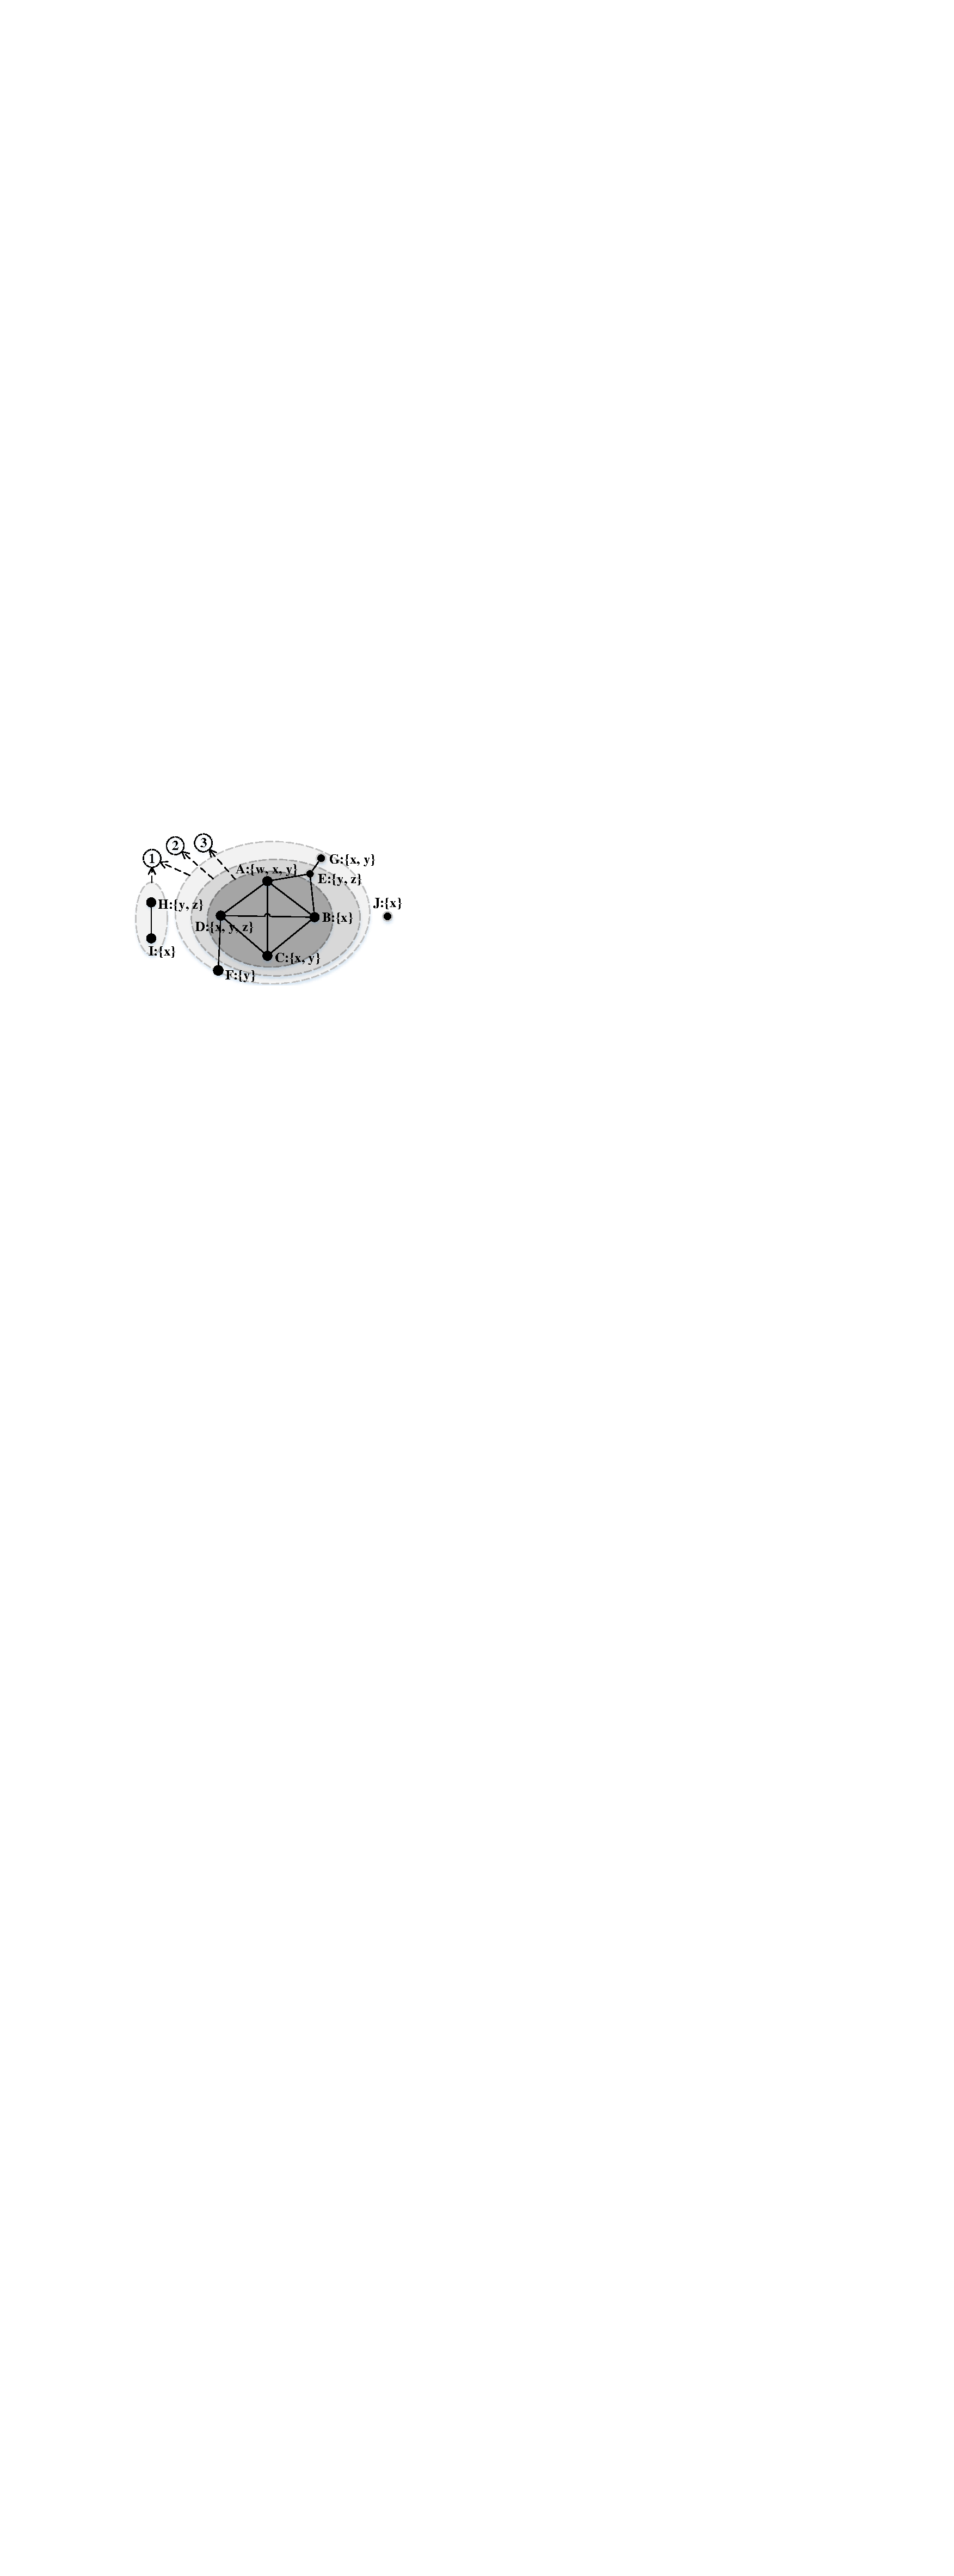
\includegraphics[width=.46\columnwidth]{figures/kcoreGraph}
            \label{fig:kcoreGraph}
        }
        \hspace{1ex}
        \subfigure[core number]{
            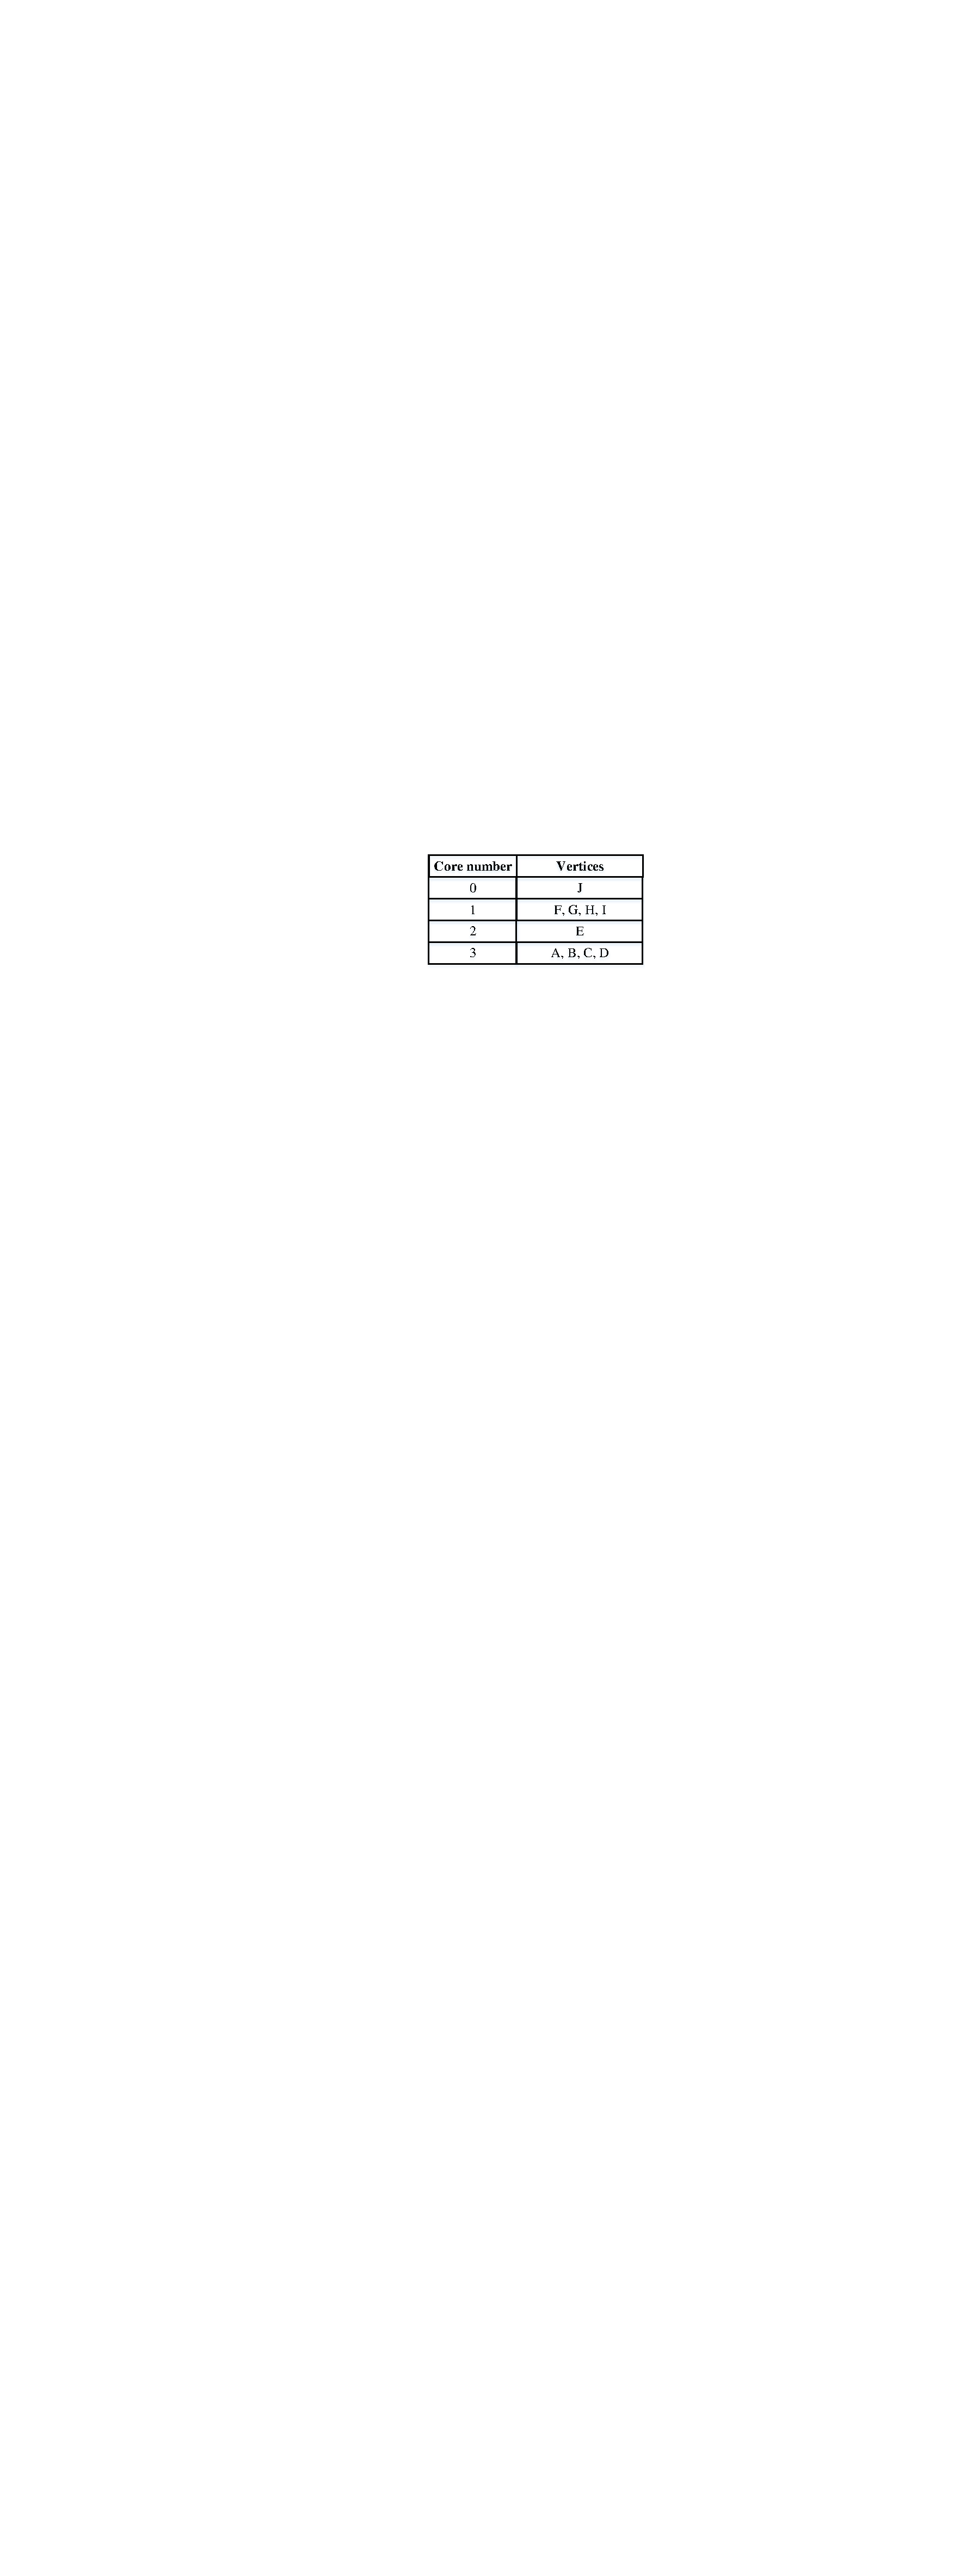
\includegraphics[width=.40\columnwidth]{figures/kcoreTable}
            \label{fig:kcoreTable}
        }
    }
    \caption{Illustrating the $k$-core and the AC.}
\end{figure}

\begin{example}
\label{eg:problem}
In Figure~\ref{fig:kcoreGraph}, $\{A,B,C,D\}$ is both a 3-core and a 3-$\widehat{core}$. The 1-core has vertices $\{A,B,C,D,E,F,G,$ $H,I\}$, and is composed of two $1$-$\widehat{core}$ components: $\{A,B,$ $C,D,E,F,G\}$ and $\{H,I\}$. The number $k$ in each circle represents the $k$-$\widehat{core}$ contained in that ellipse.
\end{example}

Observe that $k$-$core$s are ``nested''~\cite{kcore2003}: given two positive integers $i$ and $j$, if $i<j$, then $H_j \subseteq H_i$.  In Figure~\ref{fig:kcoreGraph}, $H_3$ is contained in $H_2$, which is nested in $H_1$.

\begin{definition}[Core number]
\label{def:coreNum}
Given a vertex $v \in V$, its core number, denoted by $core_G[v]$, is the highest order of a $k$-core that contains $v$.
\end{definition}

A list of core numbers and their respective vertices for Example~\ref{eg:problem} are shown in Figure~\ref{fig:kcoreTable}. In~\cite{kcore2003}, an $O(m)$ algorithm was proposed to compute the core number of every vertex.

%An efficient solution (called {\tt Global}) for finding a $k$-$\widehat{core}$ that contains a vertex $q \in V$ was presented in \cite{KDD2010}. Recently, Cui et al. have developed a fast solution called {\tt Local}~\cite{local2014}, yielding subgraph(s) of $k$-$\widehat{core}$ that satisfy structure cohesiveness. In Section~\ref{experiment}, we compare our approach with {\tt Global} and {\tt Local}.

%As discussed in Section~\ref{intro}, two vertices that do not share any keywords may still be placed together in a $k$-$\widehat{core}$. In Example~\ref{eg:problem}, $H$ and $I$ are included in the $1$-$\widehat{core}$ even though their keywords are completely different. To address this issue, we introduce the LAC search problem.

We now formally define the ACQ problem as follows.

\begin{problem}[ACQ]
\label{problem1}
Given a graph $G(V,E)$, a positive integer $k$, a vertex $q \in V$ and a set of keywords $S\subseteq W(q)$, return a set $\mathcal {G}$ of graphs, such that $\forall G_q \in \mathcal {G}$, the following properties hold:


\vspace{1ex}
$\bullet$ \textbf{Connectivity}. $G_q \subseteq G$ is connected and $q\in G_q$;

$\bullet$ \textbf{Structure cohesiveness}. $\forall$$v\in G_q$, $deg_{G_q}(v)\geq$$k$;

$\bullet$ \textbf{Keyword cohesiveness}. The size of $L(G_q, S)$ is maximal, where $L(G_q, S)=\cap_{v \in G_q}(W(v)\cap S)$ is the set of keywords shared in $S$ by all vertices of $G_q$.%\vspace{1ex}
\end{problem}

We call $G_q$ the {\it attributed community} (or AC) of $q$, and $L(G_q, S)$ the {\it AC-label} of $G_q$. In Problem~\ref{problem1}, the first two properties are also specified by the $k$-$\widehat{core}$ of a given vertex $q$~\cite{KDD2010}. The {\it keyword cohesiveness} (Property 3), which is unique to Problem~\ref{problem1}, enables the retrieval of communities whose vertices have common keywords in $S$.  We use
$S$ to impose semantics on the AC produced by Problem~\ref{problem1}. By default, $S=W(q)$, which means that the AC generated should have keywords common to those associated with $q$. If $S \subset W(q)$, it means that the ACQ user is interested in forming communities that are related to some (but not all) of the keywords of $q$. A user interface could be developed to display $W(q)$ to the user, allowing her to include the desired keywords into $S$.  For example, in Figure~\ref{fig:kcoreGraph}, if $q$=$A$, $k$=2 and $S$=$\{w,x,y\}$, the output of Problem~\ref{problem1} is $\{A,C,D\}$, with AC-label $\{x,y\}$, meaning that these vertices share the keywords $x$ and $y$.


We require $L(G_q, S)$ to be maximal in Property 3, because we wish the AC(s) returned only contain(s) the most related vertices, in terms of the number of common keywords. Let us use Figure~\ref{fig:kcoreGraph} to explain why this is important. Using the same query ($q$=$A$,$k$=2,$S$= $\{w,x,y\}$), without the ``maximal'' requirement, we can obtain communities such as $\{A,B,E\}$ (which do not share any keywords), $\{A,B,D\}$, or $\{A,B,C\}$ (which share 1 keyword). Note that there does not exist an AC with AC-label being exactly $\{w$, $x,y\}$.
Our experiments (Section~\ref{experiment}) show that imposing the ``maximal'' constraint yields the best result. Thus, we adopt Property 3 in Problem~\ref{problem1}.
If there is no AC whose vertices share one or more keywords
(\textit{i.e.}, $|L(G_q, S)|$=0), we return the subgraph of $G$ that satisfies Properties 1 and 2 only.
~\footnote{In practice, the query user can be alerted by the system when there is no sharing among the vertices.}

There are other candidates for structure cohesiveness (e.g., $k$-truss, $k$-clique) and  {\it keyword cohesiveness} (e.g., Jaccard similarity and string edit distance). An AC can also be defined in different ways. For example, an ACQ user may specify that an AC returned must have vertices that contain a specific set of keywords.
An interesting direction is to extend ACQ  to support for these criteria, and study their effectiveness.
